\documentclass{beamer}
\usepackage{amsmath}
\usepackage{amssymb}
\usepackage{physics}
\usepackage{amsthm}
\usepackage{graphicx}
\usepackage{caption}
\usepackage{subcaption}
\graphicspath{ {./figures/} }
\title{Tomografie a Radonova transformace}
\author{Dominika Hájková, Matyáš Fuksa, Ondřej Kureš}
\institute{Skupina W}
\date{2021}

\begin{document}

\frame{\titlepage}

\begin{frame}
\frametitle{Radonova transformace}
\begin{equation}
\mathcal{R}[f(\vec{x})](\rho, \theta)=_{def} \int_{-\infty}^{+\infty}f(s \vec{\theta}^\perp + \rho \vec{\theta}) \,ds
\end{equation}
\begin{equation}
\mathcal{R}[f(\vec{x})](\rho, \theta)=_{def} \int_{\vec{x}\in \mathbb{R}^2}f(\vec{x})\delta \left(\vec{x}\cdot\vec{\theta} - \rho\right) \,dv_{\vec{x}} 
\end{equation}
Ano, zde je 1. stránka této prezentace. Zde vložíme definici Radonovy transformace (nic moc složitého).
\end{frame}
\begin{frame}
\frametitle{Použití Radonovy transformace - Bod}
Překvapivě, zde je 2. stránka této prezentace. Sem bychom mohli vložit Radonovo transformaci bodu.
\end{frame}
\begin{frame}
\frametitle{Použití Radonovy transformace - Přímka}
Pro ty, co to nečekali, zde je 3. stránka této prezentace. Sem vložíme (pochopitelně) Radonovo transformaci přímky.
\end{frame}
\begin{frame}
\frametitle{Inverzní Radonova transformace}
\begin{equation}
f(\vec{x})=  \int_{\theta=0}^{\pi}
	\left\lbrace
		\mathcal{H}_{\rho \to \xi}
			\left[\frac{\partial}{\partial\rho}
				\left(\mathcal{R}[f(\vec{x})](\rho,\theta)
				\right)
			\right]
		(\xi,\theta)
	\right\rbrace
	_{\xi = \vec{x}\cdot\vec{\theta}}
	\,d\theta
\end{equation}
Ano, nikdo to neočekával, toto je 4. stránka této prezentace. Stejně jako jsme měli definici Radonovy transformace na začátku, tak stejným způsobem bychom sem mohli dát definici inverzní Radonovy transformace.
\end{frame}

\begin{frame}
\frametitle{Co snědla Vítkova dcerka?}

\begin{figure}
\centering
\begin{subfigure}{.5\textwidth}
  \centering
  
\includegraphics[width=.8\linewidth]{secret-radon.pdf}
  \label{fig:sub1}
\end{subfigure}%
\begin{subfigure}{.5\textwidth}
  \centering
  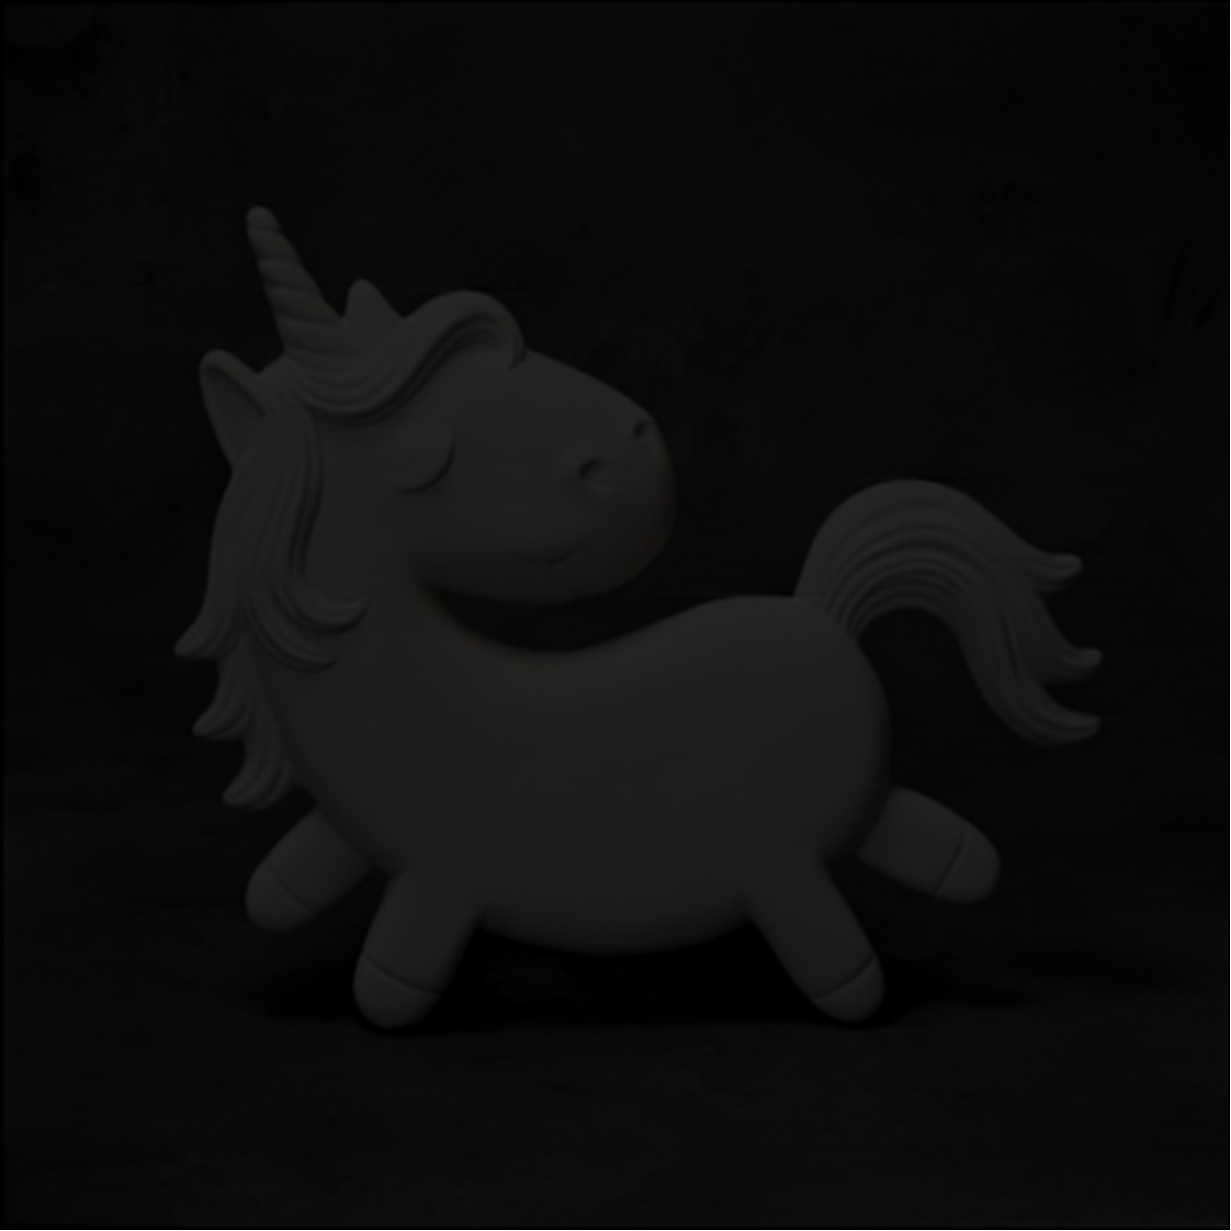
\includegraphics[width=.8\linewidth]{unicorn.pdf}
  \label{fig:sub2}
\end{subfigure}
\caption{Skrytý obrázek a odhalený obrázek}
\label{fig:test}
\end{figure}

\end{frame}
\begin{frame}
\begin{center}
\begin{huge}
Děkujeme za pozornost
\end{huge}

\end{center}

\end{frame}
\end{document}